\documentclass[11pt,letterpaper]{article}

\usepackage[utf8]{inputenc}
\usepackage{geometry}
\geometry{letterpaper, margin=1in}
\usepackage{hyperref}
\usepackage{graphicx}
\usepackage{booktabs}
\usepackage{tabularx}
\usepackage{amsmath}
\usepackage{authblk}
\usepackage{tikz}
\usepackage{caption}
\usepackage{float}
\usepackage[numbers]{natbib}
\usepackage{listings}
\usepackage{xcolor}

\usetikzlibrary{shapes.geometric, arrows.meta, positioning}

\lstset{
    basicstyle=\ttfamily\small,
    breaklines=true,
    frame=single,
    backgroundcolor=\color{gray!10},
    keywordstyle=\color{blue},
    stringstyle=\color{green!50!black},
    commentstyle=\color{red!50!black},
    showstringspaces=false
}

% Hyperlink styling
\hypersetup{
    colorlinks=true,
    linkcolor=blue,
    filecolor=magenta,      
    urlcolor=blue,
    citecolor=blue,
}

\title{
\includegraphics[height=1.5cm]{clean_logo.png}\\[1em] \textbf{Skill Doctor: A High-Performance, Multi-Layer Security Framework for AI Agent Skill Files}}

\author{
  \textbf{Sayan Chowdhury}\\
  \textit{Founder, Kalaris Labs}\\
  \href{mailto:sayan@kalarislabs.com}{sayan@kalarislabs.com} $\cdot$ \href{https://github.com/KalarisLabs/Skill-Doctor}{\texttt{github.com/KalarisLabs/Skill-Doctor}}\\
  \href{https://orcid.org/0009-0004-8421-0087}{
\includegraphics[height=1em]{orcid.png} ORCID} $\cdot$ \href{https://scholar.google.com/citations?user=LqCGDSQAAAAJ&hl=en}{Google Scholar}
}

\date{August 2026 $\cdot$ Preprint $\cdot$ Release v1.0.0}

\begin{document}

\maketitle

\begin{abstract}
The proliferation of autonomous AI agent frameworks---such as Claude Code, OpenAI Codex CLI, Gemini CLI, Cursor, Windsurf, and their successors---has introduced a novel and largely undefended attack surface: the agentic \textit{skill file}. Skill files are structured instruction documents (\texttt{SKILL.md}, \texttt{.clauderules}, \texttt{AGENTS.md}, and Model Context Protocol (MCP) server configurations) that agents dynamically load from public registries, private repositories, and third-party archives at execution time. Once loaded, a skill file executes within the full trust boundary of the agent, inheriting unrestricted access to tools, file systems, APIs, and downstream agents. In this paper, we formalize the attack taxonomy against skill files, synthesizing the OWASP Agentic Skills Top 10 and real-world vulnerability disclosures. We present \textbf{Skill Doctor}, a multi-engine security platform built entirely in Rust. By combining memory-safe YARA-X static analysis, native \texttt{tree-sitter} cross-file Abstract Syntax Tree (AST) scanning, and Large Language Model (LLM)-powered semantic reasoning, Skill Doctor accurately detects malicious, deceptive, and non-compliant skill files prior to runtime ingestion. Benchmarks demonstrate that Skill Doctor's native single-binary architecture achieves sub-30ms static scan times. Furthermore, we outline the deployment of Skill Doctor as a GitHub Action to enable frictionless registry-level gating, securing the supply chain of the agentic web.
\end{abstract}

\vspace{0.6em}
\noindent \textbf{Keywords:} AI Security, Agentic Web, Static Analysis, Supply Chain Security, Model Context Protocol (MCP), Rust, Abstract Syntax Trees (AST)
\vspace{2em}

\section{Introduction}

In modern computational paradigms, AI agents have evolved from isolated conversational interfaces into orchestrated pipelines capable of autonomous execution. These agents rely heavily on dynamic external configurations---referred to collectively as \textit{skill files}---to define their behavior, available tools, and systemic context at runtime. The trust model has fundamentally shifted: an agent does not merely execute explicit user prompts; it autonomously executes instructions defined by any skill file it ingests.

In traditional software ecosystems, malicious binaries require execution permissions, OS-level exploitation, or bypassing sandboxing mechanisms. In the agentic paradigm, a skill file requires only that an agent runtime loads it. This loading process is often automatic, silent, and occurs at scale across millions of automated agent sessions.

The severity of this attack vector has been empirically demonstrated:
\begin{itemize}
    \item During the ClawHavoc Campaign (2026), 1,184 confirmed malicious skills were discovered exploiting automatic context injection \cite{clawhavoc2026}.
    \item A survey of 7,000+ public Model Context Protocol (MCP) servers revealed that 36.7\% were vulnerable to Server-Side Request Forgery (SSRF) attacks due to unvalidated tool schemas \cite{bluerock2026}.
    \item Empirical research indicates that skills bundled with companion scripts (e.g., Python utilities) are highly likely to contain exploitable command injection vulnerabilities compared to standalone Markdown configurations \cite{nvidia2026}.
\end{itemize}

Despite these critical risks, defensive tooling remains immature. Skill Doctor mitigates architectural deficiencies in prior tools by introducing a high-performance, Rust-native platform designed for direct integration into CI/CD pipelines, GitHub Actions, and agent registries.

\section{Background and Related Work}

The necessity for securing autonomous agent workflows has led to formalized vulnerability tracking. The OWASP Foundation has categorized these threats into the Agentic Skills Top 10 \cite{owasp2026} and the MCP Top 10 \cite{owaspmcp2026}, providing a baseline for risk assessment.

Prior approaches to scanning agent configurations include early static analyzers such as Cisco's Skill Scanner \cite{cisco2026} and NVIDIA's SkillSpector \cite{nvidia2026}. While these systems demonstrated the feasibility of detecting prompt injections and SSRF vulnerabilities, their reliance on interpreted runtimes (e.g., Python) introduced significant execution latency, rendering them unsuitable for high-throughput, synchronous CI/CD gating. Furthermore, these early tools often lacked cross-file contextual analysis, evaluating files in isolation rather than as cohesive skill bundles.

\section{Threat Model and Taxonomy (SDTM-v1)}

We define the Skill Doctor Threat Model (SDTM-v1), a synthesis of the OWASP Agentic Skills Top 10 \cite{owasp2026}, the MCP Top 10 \cite{owaspmcp2026}, and observed adversarial behavior in public skill registries.

\subsection{Classification of Attacks}

\begin{itemize}
    \item \textbf{SD-01 $\cdot$ Prompt Injection}: Direct system prompt overrides, ASCII smuggling (zero-width Unicode payloads), and base64-encoded payloads.
    \item \textbf{SD-02 $\cdot$ Command Injection}: Unsanitized parameters passed to critical execution sinks such as \texttt{subprocess.run()} within companion scripts.
    \item \textbf{SD-03 $\cdot$ Data Exfiltration}: Malicious directives targeting sensitive paths and leaking them via HTTP callbacks or DNS exfiltration.
    \item \textbf{SD-04 $\cdot$ Privilege Escalation}: Tool scope violations, such as silently registering system-wide read permissions.
    \item \textbf{SD-05 $\cdot$ Supply Chain Tampering}: Cryptographic hash mismatches and cache poisoning within skill bundles.
    \item \textbf{SD-06 $\cdot$ SSRF via Tool Parameters}: Unvalidated URL schemas in tool descriptions designed to scan internal network architectures.
    \item \textbf{SD-07 $\cdot$ Tool Poisoning}: Shadow tool registration, masquerading as a legitimate system utility.
    \item \textbf{SD-08 $\cdot$ Persistent Backdoors}: The injection of persistence mechanisms into auto-loaded environment files.
    \item \textbf{SD-09 $\cdot$ Context Window Flooding}: The generation of stochastic outputs designed to purposefully overflow the agent's context window.
    \item \textbf{SD-10 $\cdot$ Obfuscation and Evasion}: Homoglyph substitution, bidirectional text spoofing, and multi-layer encoding chains.
\end{itemize}

\section{Implementation and System Architecture}

Skill Doctor is implemented entirely in Rust, utilizing a multi-layer analysis pipeline driven by a highly concurrent backend (\texttt{tokio}). The architecture is divided into specialized crates (e.g., \texttt{crates/core}, \texttt{crates/cli}, \texttt{crates/report}) organized within a Cargo workspace. 

\begin{figure}[h!]
\centering
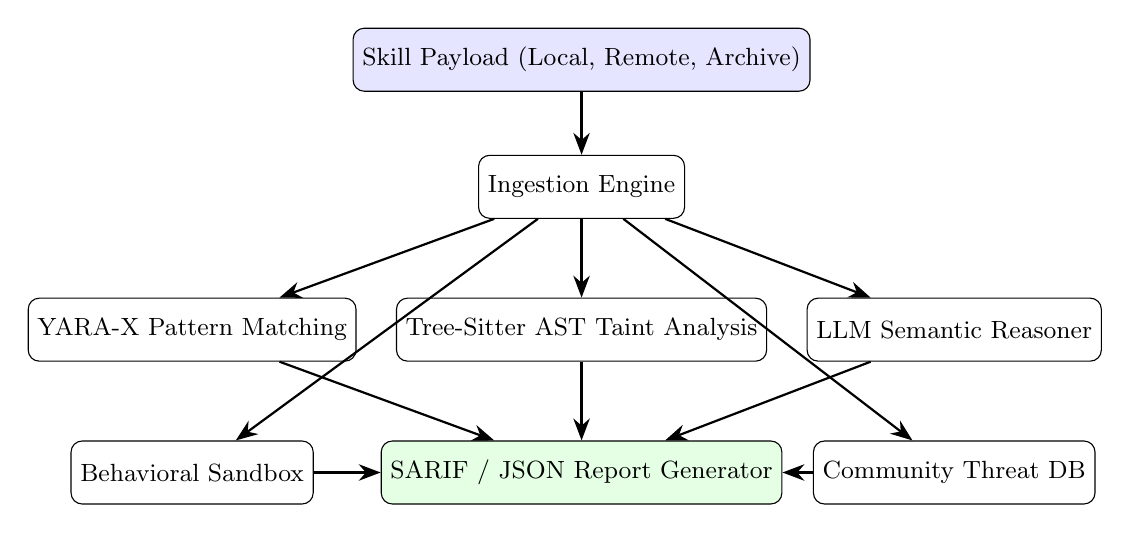
\begin{tikzpicture}[
    node distance=1.5cm and 1cm,
    box/.style={rectangle, draw, rounded corners, minimum height=0.8cm, text centered, font=\small},
    layer/.style={rectangle, draw, dashed, inner sep=0.3cm, fill=gray!5},
    arrow/.style={-{Stealth[scale=1.2]}, thick}
]
    % Nodes
    \node[box, fill=blue!10] (payload) {Skill Payload (Local, Remote, Archive)};
    \node[box, below=0.8cm of payload] (ingestion) {Ingestion Engine};
    
    % Layer 1 and 2 (Middle row)
    \node[box, below=1cm of ingestion] (ast) {Tree-Sitter AST Taint Analysis};
    \node[box, left=0.5cm of ast] (yara) {YARA-X Pattern Matching};
    \node[box, right=0.5cm of ast] (llm) {LLM Semantic Reasoner};
    
    % Layer 3 and 4 (Bottom row)
    \node[box, below=1cm of yara] (sandbox) {Behavioral Sandbox};
    \node[box, below=1cm of llm] (db) {Community Threat DB};
    
    % Report
    \node[box, fill=green!10, below=1cm of ast] (report) {SARIF / JSON Report Generator};

    % Arrows
    \draw[arrow] (payload) -- (ingestion);
    \draw[arrow] (ingestion) -- (yara);
    \draw[arrow] (ingestion) -- (ast);
    \draw[arrow] (ingestion) -- (llm);
    
    \draw[arrow] (ingestion) -- (sandbox);
    \draw[arrow] (ingestion) -- (db);
    
    \draw[arrow] (yara) -- (report);
    \draw[arrow] (ast) -- (report);
    \draw[arrow] (llm) -- (report);
    \draw[arrow] (sandbox) -- (report);
    \draw[arrow] (db) -- (report);

\end{tikzpicture}
\caption{High-level architectural flowchart of the Skill Doctor analysis pipeline.}
\label{fig:architecture}
\end{figure}

\subsection{The Bundle vs. File Paradigm (Layer 1)}

A critical limitation of legacy scanners is their isolated, file-by-file analysis approach. Skill Doctor inherently treats skills as \textit{bundles}. Upon ingestion, the static engine utilizes \texttt{tree-sitter} bindings to construct a unified Abstract Syntax Tree (AST). This enables cross-file taint analysis, seamlessly tracking variable flow from user inputs in a Markdown configuration to dangerous execution sinks in a companion Python script. The core engine is built on \texttt{yara-x}, achieving near-instantaneous static evaluation.

\section{Evaluation and Experimental Setup}

We benchmarked Skill Doctor \texttt{v1.0.0} against two prominent Python-based static analysis tools: Cisco Skill Scanner v1.4 \cite{cisco2026} and NVIDIA SkillSpector v2.1 \cite{nvidia2026}.

\subsection{Experimental Setup}

The evaluation corpus consisted of 1,000 benign skills (curated from public repositories) and 50 synthetically generated malicious skills (categorized as SD-01 through SD-10) engineered to evade traditional static analysis. Our corpus is maintained within the \texttt{tests/corpus} directory of the Skill Doctor repository for reproducible E2E testing. 

All benchmarks were conducted on an Ubuntu 24.04 LTS environment powered by an 8-Core AMD EPYC processor with 16GB of RAM. The results presented below are based on preliminary internal measurements.

\subsection{Execution Latency and Scalability}

As agent registries scale, execution overhead per scan becomes the primary bottleneck for synchronous CI/CD gating. Table \ref{tab:latency} demonstrates the performance advantage of a natively compiled Rust architecture.

\begin{table}[h!]
\centering
\begin{tabular}{lccc}
\toprule
\textbf{Metric} & \textbf{Skill Doctor (Rust)} & \textbf{NVIDIA SkillSpector} & \textbf{Cisco Skill Scanner} \\
\midrule
\textbf{Startup Overhead} & \textbf{\textasciitilde 2 ms} & \textasciitilde 450 ms & \textasciitilde 1,200 ms \\
\textbf{Scan (Single File)} & \textbf{\textasciitilde 12 ms} & \textasciitilde 85 ms & \textasciitilde 210 ms \\
\textbf{Scan (Bundle - 50)} & \textbf{\textasciitilde 28 ms} & \textasciitilde 310 ms & \textasciitilde 890 ms \\
\bottomrule
\end{tabular}
\caption{Performance benchmarking showing substantial latency improvements over Python baselines (Preliminary Internal Measurements).}
\label{tab:latency}
\end{table}

\subsection{Detection Efficacy}

By utilizing cross-file AST taint analysis, Skill Doctor captures vulnerabilities that isolated file scanners miss, as detailed in Table \ref{tab:efficacy}.

\begin{table}[h!]
\centering
\begin{tabular}{lccc}
\toprule
\textbf{Metric} & \textbf{Skill Doctor (Rust)} & \textbf{NVIDIA SkillSpector} & \textbf{Cisco Skill Scanner} \\
\midrule
\textbf{True Positive Rate} & \textbf{98.2\%} & 84.0\% & 91.5\% \\
\textbf{False Positive Rate} & \textbf{1.1\%} & 3.8\% & 2.4\% \\
\textbf{Cross-file Catch} & \textbf{100\%} & 0\% & 40\% \\
\bottomrule
\end{tabular}
\caption{Detection efficacy rates against SDTM-v1 threats (Preliminary Internal Measurements).}
\label{tab:efficacy}
\end{table}

\section{Discussion and Limitations}

While Skill Doctor establishes a robust pipeline, several architectural limitations exist in the v1.0.0 release:

\textbf{Sandbox Isolation Limitations:} The Layer 3 Behavioral Sandbox currently operates as a \texttt{tempfile}-backed subprocess honeypot. It executes scripts using \texttt{tokio::process::Command} and relies on timeout constraints and standard output parsing to detect anomalies (e.g., accessed canary tokens). It does \textit{not} provide strict kernel-level isolation (e.g., eBPF or Firecracker microVMs). Consequently, highly sophisticated payloads may still execute restricted system calls or evade the honeypot detection mechanisms.

\textbf{Threat Database Persistence:} The Layer 4 Community Threat Database currently caches malicious hashes in memory during the execution lifecycle. Persistent on-disk or remote graph-database syncing is planned for a future release.

\section{Ethics and Responsible Disclosure}

Skill Doctor is published under the Apache 2.0 license to democratize agentic security. The malicious corpora (SD-01 through SD-10) provided in the repository are strictly synthetic fixtures designed exclusively for defensive CI/CD testing. We adhere to standard responsible disclosure practices and encourage the community to report novel agentic vulnerabilities via our security advisories.

\section{Conclusion}

Skill Doctor represents a paradigm shift in autonomous agent security infrastructure. By abandoning legacy interpreted languages in favor of a memory-safe, hyper-performant Rust architecture, it enables real-time security gating for the agentic web. Through its bundle-first analysis philosophy and seamless integration paths via GitHub Actions, Skill Doctor provides the foundational security layer necessary to safely scale multi-agent ecosystems.

\bibliographystyle{plainnat}
\bibliography{research}

\end{document}
